\documentclass[aspectratio=169]{beamer}

\mode<presentation>
{
  \usetheme{default}
  \usecolortheme{default}
  \usefonttheme{default}
  \setbeamertemplate{navigation symbols}{}
  \setbeamertemplate{caption}[numbered]
  \setbeamertemplate{footline}[frame number]  % or "page number"
  \setbeamercolor{frametitle}{fg=white}
  \setbeamercolor{footline}{fg=black}
} 

\usepackage[english]{babel}
\usepackage[utf8x]{inputenc}
\usepackage{tikz}
\usepackage{courier}
\usepackage{array}
\usepackage{bold-extra}
\usepackage{minted}
\usepackage[thicklines]{cancel}

\xdefinecolor{dianablue}{rgb}{0.18,0.24,0.31}
\xdefinecolor{darkblue}{rgb}{0.1,0.1,0.7}
\xdefinecolor{darkgreen}{rgb}{0,0.5,0}
\xdefinecolor{darkgrey}{rgb}{0.35,0.35,0.35}
\xdefinecolor{darkorange}{rgb}{0.8,0.5,0}
\xdefinecolor{darkred}{rgb}{0.7,0,0}
\definecolor{darkgreen}{rgb}{0,0.6,0}
\definecolor{mauve}{rgb}{0.58,0,0.82}

\title[2018-04-30-paris-oamap]{Object-array mapping and columnar data granularity}
\author{Jim Pivarski}
\institute{Princeton University -- DIANA-HEP}
\date{April 30, 2018}

\begin{document}

\logo{\pgfputat{\pgfxy(0.11, 7.4)}{\pgfbox[right,base]{\tikz{\filldraw[fill=dianablue, draw=none] (0 cm, 0 cm) rectangle (50 cm, 1 cm);}\mbox{\hspace{-8 cm}
\includegraphics[height=1 cm]{princeton-logo-long.png}
\includegraphics[height=1 cm]{diana-hep-logo-long.png}}}}}

\begin{frame}
  \titlepage
\end{frame}

\logo{\pgfputat{\pgfxy(0.11, 7.4)}{\pgfbox[right,base]{\tikz{\filldraw[fill=dianablue, draw=none] (0 cm, 0 cm) rectangle (50 cm, 1 cm);}\mbox{\hspace{-8 cm}
\includegraphics[height=1 cm]{princeton-logo.png}
\includegraphics[height=1 cm]{diana-hep-logo.png}}}}}

% Uncomment these lines for an automatically generated outline.
%\begin{frame}{Outline}
%  \tableofcontents
%\end{frame}

% START START START START START START START START START START START START START

\begin{frame}{Context}
\vspace{0.35 cm}
\begin{columns}[t]
\column{0.4\linewidth}
\underline{High Performance Computing (HPC)}

\vspace{0.15 cm}
\begin{itemize}
\item A lot of focus on data contiguity, CPU cache efficiency, and vectorization.
\item Data structures are often converted to flat arrays or tables, making it easier to reason about such issues.
\end{itemize}

\column{0.56\linewidth}
\begin{uncoverenv}<2->
\underline{High Energy Physics (HEP)}

\vspace{0.15 cm}
\begin{itemize}
\item Data structures are generally:

\begin{center}
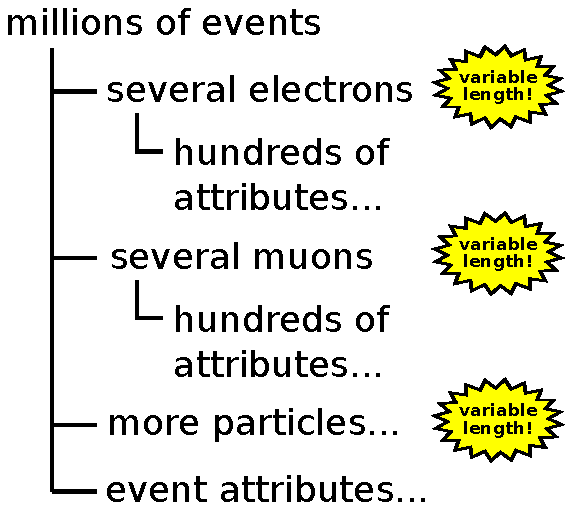
\includegraphics[width=0.7\linewidth]{event-structure.pdf}
\end{center}

\item Analysis code is branchy and pointer-heavy;

``Looks more like string processing!''
\end{itemize}
\end{uncoverenv}
\end{columns}
\end{frame}

\begin{frame}{Context}
\vspace{0.25 cm}
Preparing data for analysis consists of {\it copying} parts of the centrally produced dataset.

\vspace{0.25 cm}
The choice of events to ``skim'' and attributes to ``slim'' must be made before interactive (human-timescale) data exploration becomes possible.

\vspace{0.25 cm}
Disk space needs will skyrocket in the High-Luminosity LHC (HL-LHC) era.

\vspace{0.5 cm}
\begin{columns}[c]
\column{0.5\linewidth}
\mbox{ } \hfill 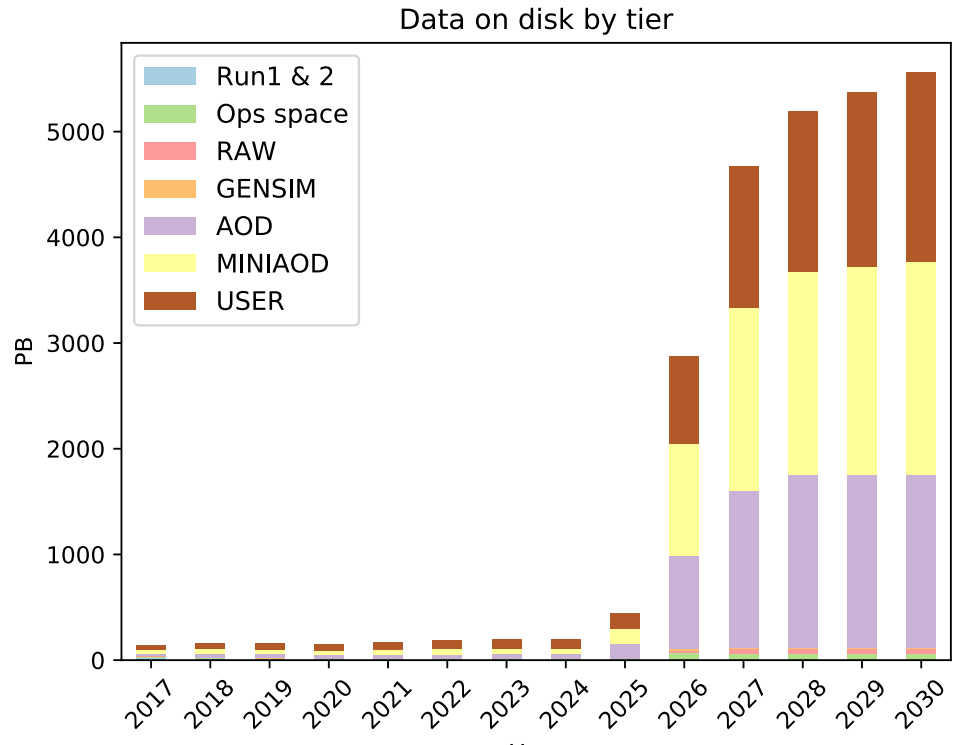
\includegraphics[height=4.5 cm]{cms-data-explosion.png}

\column{0.5\linewidth}

\vspace{0.2 cm}
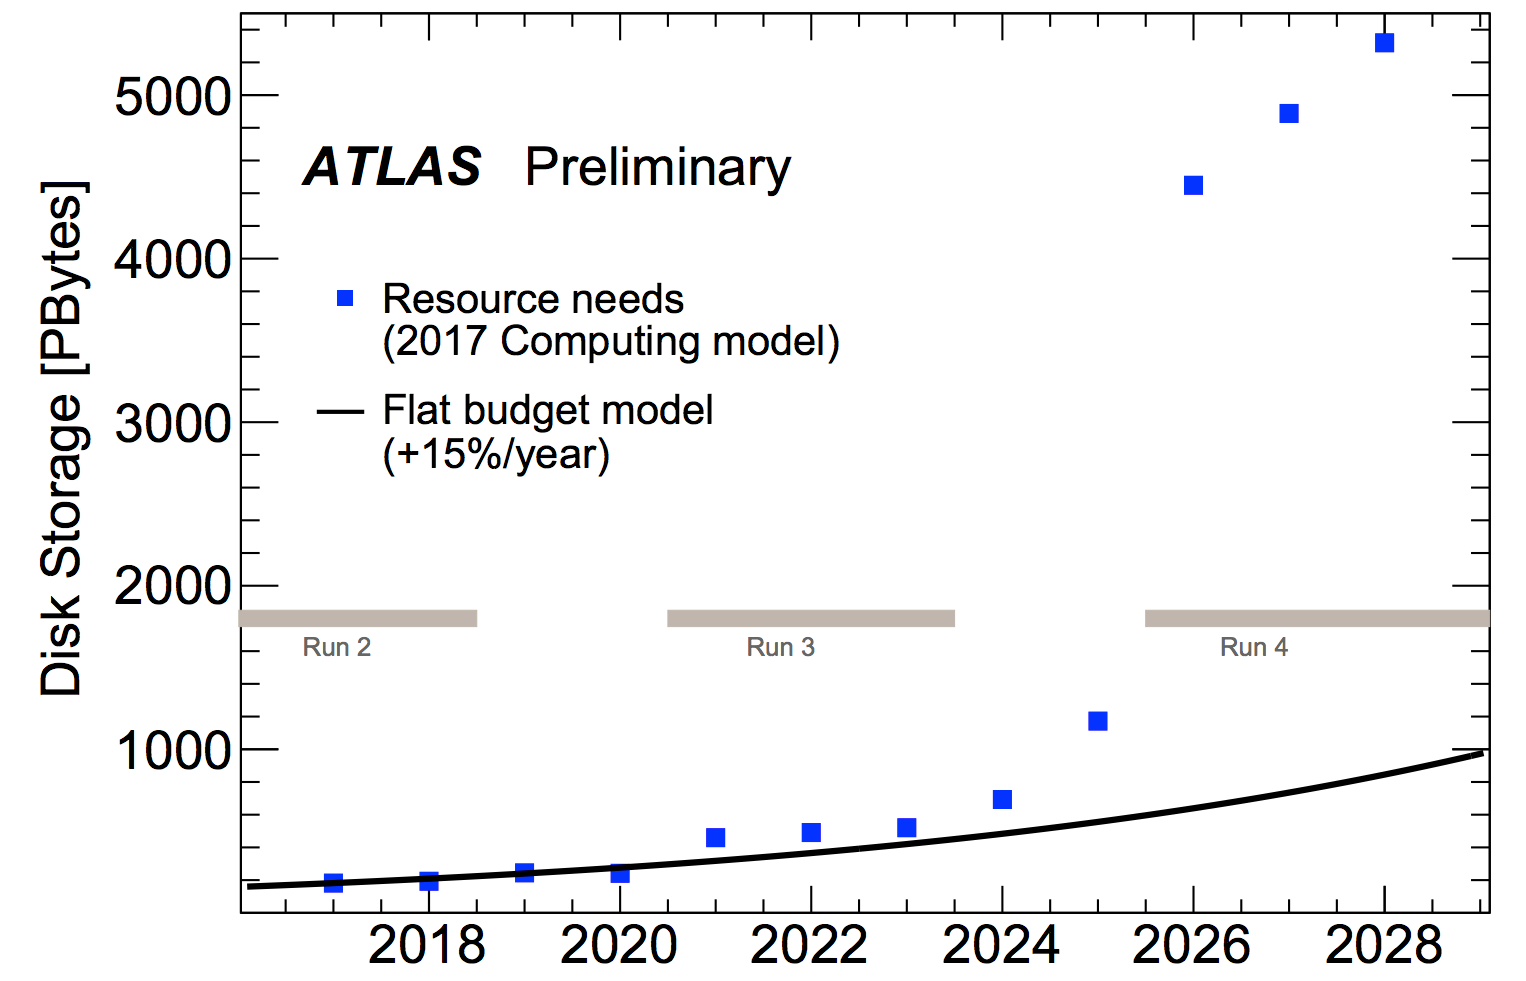
\includegraphics[height=4.4 cm]{atlas-data-explosion.png} \hfill \mbox{ }
\end{columns}
\end{frame}

\begin{frame}{Context}
\vspace{0.75 cm}
\begin{itemize}\setlength{\itemsep}{0.75 cm}
\item[$\rightarrow$]<1-> Several projects are underway to rewrite or rethink core reconstruction algorithms: vectorized tracking, machine learning-based pattern recognition\ldots

\item[$\rightarrow$]<2-> But event reconstruction isn't everything; there's also data analysis!

\vspace{0.1 cm}
\begin{itemize}\setlength{\itemsep}{0.15 cm}
\item<3-> not centrally produced: code written by ``users'' of the data
\item<4-> ad-hoc (``if we knew what we were doing, it wouldn't be called research'')
\item<5-> should be focused on physics and statistics issues, not computing
\end{itemize}
\end{itemize}
\end{frame}

\begin{frame}{New technique}
\vspace{0.35 cm}
\textcolor{darkblue}{\large \underline{Object-array mapping (OAMap)}}

\vspace{0.15 cm}
\begin{itemize}\setlength{\itemsep}{0.15 cm}
\item Let data analysts write traditional object-oriented code, but translate it to HPC-like array operations at runtime (generalization of AOS $\to$ SOA).
\item<2-> Analogy with object-relational mapping (ORM), but for low-level arrays.
\item<3-> Represent nested, variable-length object data as (unequal length) arrays of each attribute and {\it never deserialize} them into runtime objects.
\item<4-> Two ways of doing this:

\vspace{0.05 cm}
\begin{description}\setlength{\itemsep}{0.1 cm}
\item[proxies]<5-> that simulate objects on the fly by accessing array data in response to attribute references (for low-latency exploration).
\item[compilation]<6-> that replaces user code with code that accesses array elements directly (for high-throughput processing).
\end{description}
\end{itemize}

\vspace{0.2 cm}
\begin{uncoverenv}<7->
\begin{minipage}{\linewidth}
\scriptsize \textcolor{darkblue}{Prior art:} T.\ Mattis, J.\ Henning, P.\ Rein, R.\ Hirschfeld, M.\ Appeltauer, ``Columnar Objects: Improving the Performance of Analytical Applications,'' in {\it 2015 ACM International Symposium on New Ideas, New Paradigms, and Reflections on Programming and Software (Onward!),} 2015, pp.\ 197--210.
\end{minipage}
\end{uncoverenv}
\end{frame}

\begin{frame}{Not new: splitting complex data into columns}
\vspace{0.35 cm}
\textcolor{darkblue}{\large Example:} {\tt List\big(List\big(Record\big(\{"x":\ "char", "y":\ "int"\}\big)\big)\big)}

\vspace{0.25 cm}
\begin{tabular}{r l}
\small logical data & {\tt\scriptsize \textcolor{blue}{[}\textcolor{violet}{[}(\textcolor{darkorange}{a},\textcolor{darkgreen}{1}), (\textcolor{darkorange}{b},\textcolor{darkgreen}{2}), (\textcolor{darkorange}{c},\textcolor{darkgreen}{3}), (\textcolor{darkorange}{d},\textcolor{darkgreen}{4})\textcolor{violet}{]}, \textcolor{violet}{[]}, \textcolor{violet}{[}(\textcolor{darkorange}{e},\textcolor{darkgreen}{5}), (\textcolor{darkorange}{f},\textcolor{darkgreen}{6})\textcolor{violet}{]}\textcolor{blue}{]}, \textcolor{blue}{[]}, \textcolor{blue}{[}\textcolor{violet}{[}(\textcolor{darkorange}{g},\textcolor{darkgreen}{7})\textcolor{violet}{]}\textcolor{blue}{]}\ \textcolor{white}{]}} \\\hline
\small outer list stops & {\tt\scriptsize \textcolor{blue}{[\ \ \ \ \ \ \ \ \ \ \ \ \ \ \ \ \ \ \ \ \ \ \ \ \ \ \ \ \ \ \ \ \ \ \ \ \ \ \ \ \ \ \ \ \ \ \ \ 3,\ \ 3,\ \ \ \ \ \ \ \ \ 4]}} \\
\small inner list stops & {\tt\scriptsize \textcolor{violet}{[\ \ \ \ \ \ \ \ \ \ \ \ \ \ \ \ \ \ \ \ \ \ \ \ \ \ \ 4,\ \ 4,\ \ \ \ \ \ \ \ \ \ \ \ \ \ 6,\ \ \ \ \ \ \ \ \ \ \ \ \ 7\ ]}} \\
\small ``x'' attribute & {\tt\scriptsize \textcolor{darkorange}{[\ \ a,\ \ \ \ \ b,\ \ \ \ \ c,\ \ \ \ \ d,\ \ \ \ \ \ \ \ \ \ \ e,\ \ \ \ \ f,\ \ \ \ \ \ \ \ \ \ \ \ \ g\ \ \ \ \ ]}} \\
\small ``y'' attribute & {\tt\scriptsize \textcolor{darkgreen}{[\ \ \ \ 1,\ \ \ \ \ 2,\ \ \ \ \ 3,\ \ \ \ \ 4,\ \ \ \ \ \ \ \ \ \ \ 5,\ \ \ \ \ 6,\ \ \ \ \ \ \ \ \ \ \ \ \ 7\ \ \ ]}}
\end{tabular}

\vspace{0.35 cm}
\begin{uncoverenv}<2->
\textcolor{darkblue}{\large Transformation rules:}
\begin{itemize}
\item Primitive data at leaves of schema are stored contiguously, without structure.
\item List structure encoded in a separate ``stops'' array, computed from the cumulative number of entries at its level of depth, written at each closing bracket.
\end{itemize}
\end{uncoverenv}

\vspace{0.1 cm}
\begin{uncoverenv}<3->
\textcolor{darkblue}{\large Variations:}
\begin{itemize}
\item Store list structure as combined ``starts'' and ``stops'': {\tt\small [0, 4, 4, 6, 7]}
\item Store as list lengths instead (better varint packing, but not randomly accessible).
\item Dremel/Parquet's definition levels and repetition levels (same issue).
\end{itemize}
\end{uncoverenv}
\end{frame}

\begin{frame}{Also not new: performing runtime calculations on columns}
\vspace{0.3 cm}

\includegraphics[width=\linewidth]{apache-arrow.png}
\end{frame}

\begin{frame}[fragile]{\textcolor{yellow}{\bf New:} viewing split array data as objects for general-purpose code}
\vspace{0.1 cm}
\small
\begin{minted}{python}
>>> for event in events:
...     print(event)
...     for mu in event.Muon:
...         print("    {} {} {} {}".format(mu, mu.pt, mu.eta, mu.phi))
...
<Event at index 0>
<Event at index 1>
    <Muon at index 0> 4.00707864761 -0.517944335938 0.292175292969
<Event at index 2>
    <Muon at index 1> 49.4589920044 0.439025878906 -2.16455078125
    <Muon at index 2> 3.01149749756 -1.42895507812 -0.00624084472656
<Event at index 3>
<Event at index 4>
    <Muon at index 3> 4.55658817291 0.792846679688 1.30639648438
<Event at index 5>
    <Muon at index 4> 96.6624984741 -1.40112304688 2.5771484375
    <Muon at index 5> 11.0187826157 -1.71313476562 -2.58740234375
    <Muon at index 6> 4.674451828 -0.969848632812 0.640625
\end{minted}

\vspace{-5.5 cm}
\begin{uncoverenv}<2->
\begin{center}
\fcolorbox{black}{white}{\begin{minipage}{0.8\linewidth}
\vspace{0.25 cm}
\begin{center}
\begin{minipage}{0.9\linewidth}
These {\tt\small events} are proxies that fetch list stops on demand and each {\tt\small mu} fetches data from {\tt\small pt}, {\tt\small eta}, and {\tt\small phi} arrays on demand.

\vspace{0.25 cm}
No restriction on programming model--- any loops, function calls, branching, etc. are allowed.
\end{minipage}
\end{center}
\vspace{-0.1 cm}
\end{minipage}}
\end{center}
\end{uncoverenv}
\vspace{5.5 cm}

\vspace{-10.6 cm}
\hfill \uncover<3->{\fbox{\normalsize e.g.\ for Pandas {\tt\small DataFrame.apply(fcn)}}}
\vspace{10.6 cm}
\end{frame}

\begin{frame}[fragile]{\textcolor{yellow}{\bf New:} compiling that code to eliminate temporary proxies}
\vspace{0.15 cm}
\scriptsize
\begin{minted}{python}
>>> import numpy
>>> import numba

>>> @numba.njit                 # declares the following function to be compiled
... def compute(events, out):   # proxies can be passed in/out of compiled functions
...     i = 0
...     for event in events:    # "event" and "event.Muon" lists are a compiler fiction
...         if len(event.Muon) == 2:
...             mu1, mu2 = event.Muon[0], event.Muon[1]
...             px = mu1.px + mu2.px
...             py = mu1.py + mu2.py
...             pz = mu1.pz + mu2.pz
...             energy = mu1.energy + mu2.energy
...             out[i] = sqrt(energy**2 - px**2 - py**2 - pz**2)
...             i += 1

>>> out = numpy.empty(1921077)
>>> compute(events, out)        # compilation and array-fetching happen on first call
                                # but before execution

>>> out
array([90.22780609, 74.74654388, 89.75765991, ..., 92.06494904,
       85.44384003, 75.96061707])
\end{minted}
\end{frame}

\begin{frame}{What's happening here?}
\vspace{0.4 cm}

\textcolor{darkblue}{\large Strongly typed schema:}
\begin{itemize}
\item Primitives, lists, unions (sum types), records \& tuples (product types), pointers.
\item Describes structure and also maps elements onto array names.
\end{itemize}

\vspace{0.25 cm}
\begin{uncoverenv}<2->
\textcolor{darkblue}{\large Proxy objects:}
\begin{itemize}
\item Maintain references to a dict of arrays (or equivalent) and subelement generators.
\item Overload {\tt\small \_\_getattr\_\_} and {\tt\small \_\_getitem\_\_} to generate subelement proxies or values.
\end{itemize}
\end{uncoverenv}

\begin{uncoverenv}<3->
\vspace{0.25 cm}
\textcolor{darkblue}{\large Type-inferring compiler pass:}
\begin{itemize}
\item Static type-safety checked against the schema.
\item Identifies a minimal set of arrays to fetch: load only the columns you need.
\end{itemize}
\end{uncoverenv}

\begin{uncoverenv}<4->
\vspace{0.25 cm}
\textcolor{darkblue}{\large Lowering compiler pass:}
\begin{itemize}
\item Each object gets replaced by an integer index, passed on the stack.
\item Equivalent of {\tt\small \_\_getattr\_\_} and {\tt\small \_\_getitem\_\_} emitted as LLVM pointer arithmetic.
\end{itemize}
\end{uncoverenv}
\end{frame}

\begin{frame}[fragile]{Implemented in Python as Numba extensions}
\vspace{0.15 cm}
\scriptsize
\begin{minted}{python}
@nb.typing.templates.infer
class ListProxyGetItem(nb.typing.templates.AbstractTemplate):
    key = "getitem"
    def generic(self, args, kwds):
       if len(args) == 2:
          tpe, idx = args
          if isinstance(tpe, ListProxyNumbaType) and isinstance(idx, nb.types.Integer):
             return typeof_generator(tpe.generator.content)(tpe, idx)

@nb.extending.lower_builtin("getitem", ListProxyNumbaType, nb.types.Integer)
def listproxy_getitem(context, builder, sig, args):
    listtpe, indextpe = sig.args; listval, indexval = args
    listproxy = nb.cgutils.create_struct_proxy(listtpe)(context, builder, listval)
    indexval = cast_int64(builder, indexval)

    normindex_ptr = nb.cgutils.alloca_once_value(builder, indexval)
    with builder.if_then(builder.icmp_signed("<", indexval, literal_int64(0))):
        builder.store(builder.add(indexval, listproxy.length), normindex_ptr)
    normindex = builder.load(normindex_ptr)

    at = builder.add(listproxy.whence, builder.mul(listproxy.stride, normindex))
    return generate(context, builder, listtpe.generator.content, listproxy.baggage,
                    listproxy.ptrs, listproxy.lens, at)
\end{minted}
\end{frame}

\begin{frame}[fragile]{Operations on OAMap data}
\vspace{0.3 cm}
Because of heavy reliance on indexes, OAMap data can only be {\it appended} in constant time (assuming arrays/files can grow). In HEP, we'd treat them as immutable.

\small
\begin{uncoverenv}<2->
\begin{minted}{python}
>>> def compute_pz(muon):
...     return muon.pt * math.sinh(muon.eta)
>>> events_v2 = events.define("pz", compute_pz, at="Muon")
\end{minted}
\end{uncoverenv}
\begin{uncoverenv}<3->
\begin{minted}{python}
>>> events_v2[1].Muon[0].pz
-2.1694915
>>> events_v2.project("Muon/pz")
[[], [-2.1694915], [], [], [-6.8923326], ...,
 [10.54625], [10.16687], [], [-9.802038], [-85.11946]]
\end{minted}
\end{uncoverenv}
\begin{uncoverenv}<4->
\begin{minted}{python}
>>> events_v3 = events_v2.filter(lambda event: len(event.Muon) >= 2)
>>> events_v3.project("Muon/pz")
[[22.418062, -5.9247837], [-184.30815, -29.56351, -5.278402], ...,
 [34.093197, -18.383192, -8.172784], [-10.909517, 2.486978]]
>>> len(events), len(events_v2), len(events_v3)
(1921077, 1921077, 299751)
\end{minted}
\end{uncoverenv}
\end{frame}

\begin{frame}[fragile]{Operations (like {\tt define}) change schema, add new arrays}
\vspace{0.15 cm}
\scriptsize
\begin{minted}{python}
>>> events_v2.schema.show()
List(
  starts = 'object-B',
  stops = 'object-E',
  doc = 'Events',
  content = Record(
    name = 'Event',
    fields = {
      'Muon': List(
        starts = 'nMuon',
        stops = 'nMuon',
        content = Record(
          name = 'Muon',
          fields = {
            'pt': Primitive(dtype('float32'), data='Muon_pt'),
            'eta': Primitive(dtype('float32'), data='Muon_eta'),
            'phi': Primitive(dtype('float32'), data='Muon_phi'),
            ...                           # all the old schema fields plus one new one
            'pz': Primitive(dtype('float32'), data='array-0', namespace='namespace-0'),
          })
      ),
      ...
    }))
\end{minted}

\vspace{-7.7 cm}
\hfill \begin{minipage}{0.6\linewidth}
\begin{minted}{python}
>>> events_v2._arrays.namespace
'namespace-0'
>>> events_v2._arrays.new
{'array-0':
     array([-2.1694915,  -6.8923326, -109.195724 , ...,
            -9.802038 , -85.11946  ], dtype=float32)}
\end{minted}

\begin{uncoverenv}<2->
\normalsize
Original dataset: 3482~MB

\vspace{0.2 cm}
Original $+$ derived: 3482~MB + 5.2~MB
\end{uncoverenv}
\end{minipage}
\vspace{7.7 cm}
\end{frame}

\begin{frame}[fragile]{Operations (like {\tt filter}) change schema, add new arrays}
\vspace{0.15 cm}
\scriptsize
\begin{minted}{python}
>>> events_v3.schema.show()
List(
  starts = 'array-0',
  stops = 'array-1',
  namespace = 'namespace-1',
  doc = 'Events',
  content = Pointer(
    positions = 'array-2',
    namespace = 'namespace-1',
    target = Record(
      name = 'Event',
      fields = {
        'Muon': List(
          starts = 'nMuon',
          stops = 'nMuon',
          content = Record(
            name = 'Muon',
            ...
            )
        ),
        ...
      })
  ))
\end{minted}
\vspace{-7.7 cm}
\hfill \begin{minipage}{0.6\linewidth}
\begin{minted}{python}
>>> events_v3._arrays.namespace
'namespace-1'
>>> events_v3._arrays.new
{'array-0': array([0]),
 'array-1': array([299751]),
 'array-2': array([     13,      16,      17, ...,
                   1921064, 1921065, 1921070])}
                   # using pointers as an event list
\end{minted}

\begin{uncoverenv}<2->
\normalsize
Original dataset: 3482~MB

\vspace{0.2 cm}
Original $+$ derived: 3482~MB + 0.41~MB
\end{uncoverenv}

\vspace{1 cm}
\begin{uncoverenv}<3->
\Large ``Soft'' skims are essentially free.
\end{uncoverenv}
\end{minipage}
\vspace{7.7 cm}
\end{frame}

\begin{frame}{Columnar granularity}
\vspace{0.25 cm}

\begin{columns}[c]
\column{0.4\linewidth}
\begin{itemize}
\item AOD (Analysis Object Data) was intended for analysis
\item MiniAOD is a copy with derived products ({\tt\small define})
\item USER are hundreds of skims made by physicists ({\tt\small filter})
\end{itemize}

\vspace{0.25 cm}
\uncover<2->{If we could access columns of data \`a la carte the way OAMap does, we could support many versions of the data with only one copy.}

\vspace{0.25 cm}
\uncover<3->{\small \textcolor{darkblue}{The catch:} soft skims and structural sharing only work if the data reside on a shared service, which would be a culture shift in HEP.}

\column{0.6\linewidth}
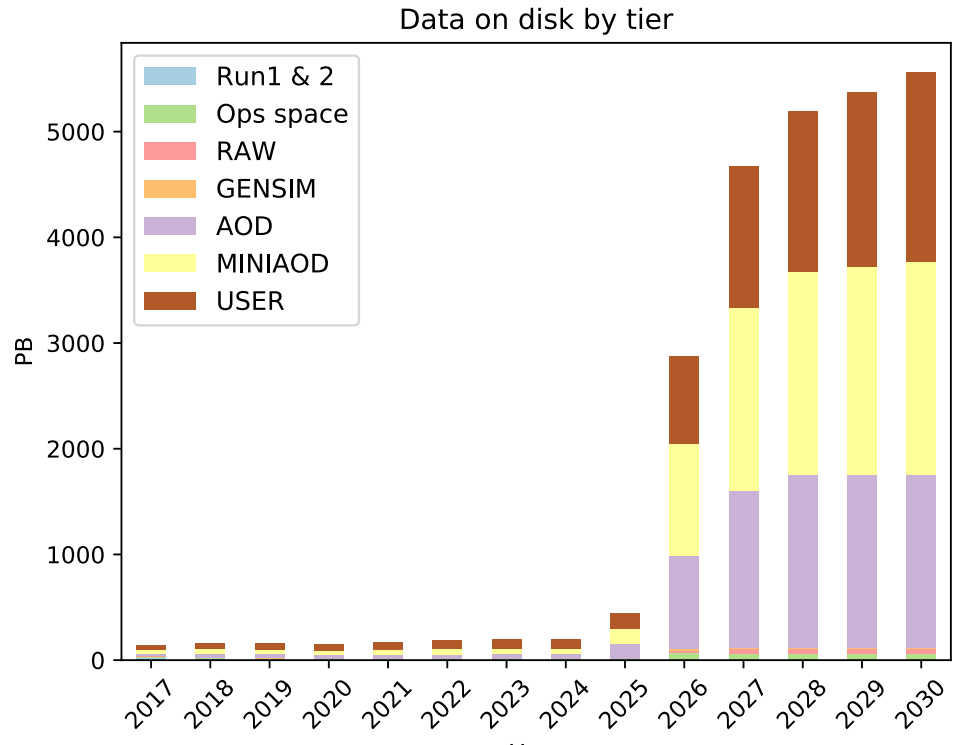
\includegraphics[width=\linewidth]{cms-data-explosion.png}
\end{columns}
\end{frame}

\begin{frame}{Culture shift: analysis in a database-like query system}
\vspace{0.5 cm}

\begin{center}
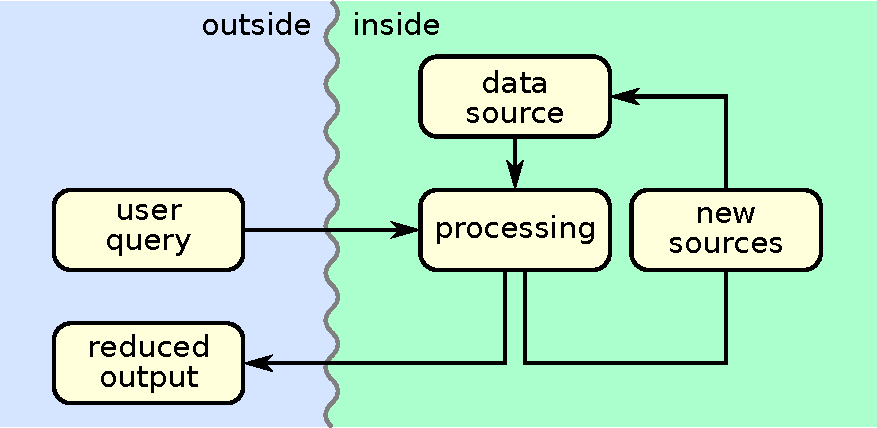
\includegraphics[width=0.65\linewidth]{basic-block-diagram.pdf}
\end{center}

\begin{itemize}
\item Large datasets (centrally produced and user derivations) have to live inside a service for index-based links to remain useful.
\item User interactions would become a series of queries $\to$ reduced outputs.
\end{itemize}
\end{frame}

\begin{frame}{OAMap status (last slide)}
\vspace{0.5 cm}
\large
\begin{itemize}\setlength{\itemsep}{0.5 cm}
\item Data types and their array representations \hfill \textcolor{darkorange}{\bf done\hspace{-0.15 cm}}
\begin{itemize}
\item {\it except:} will probably revisit masks to make them more like Arrow's
\end{itemize}

\item Python proxies and compilation as a Numba extension \hfill \textcolor{darkorange}{\bf done}

\item Other language versions (C++, Julia) \hfill \textcolor{darkorange}{\bf thinking about it}

\item Functional operations (e.g.\ {\tt\normalsize define, filter}) \hfill \textcolor{darkorange}{\bf alpha version}

\item Columnar granularity \hfill \textcolor{darkorange}{\bf alpha version}

\item Delayed operations, distributed processing (with Dask) \hfill \textcolor{darkorange}{\bf in development}

\vspace{0.15 cm}
``Partitions'' of big lists (split at entry boundaries for parallel processing).
\end{itemize}
\end{frame}

\end{document}
